\documentclass[conference]{IEEEtran}
\usepackage{CJKutf8}
\usepackage{cite}
\usepackage{amsmath,amssymb,amsfonts}
\usepackage{algorithmic}
\usepackage{graphicx}
\usepackage{textcomp}
\usepackage{xcolor} 
\usepackage{multirow}
\def\BibTeX{{\rm B\kern-.05em{\sc i\kern-.025em b}\kern-.08em
    T\kern-.1667em\lower.7ex\hbox{E}\kern-.125emX}}
\begin{document} 
\begin{CJK}{UTF8}{bsmi}

\title{HW1 - GA in Numerical Optimization}
 
\author{
\IEEEauthorblockN{Sheng-Hsuan Peng}
\IEEEauthorblockA{
\textit{PME, NTHU} \\
107033588}}

\maketitle

\section{Objectives}
Practice and get familiar with the most widely used evolutionary algorithm — genetic algorithm
(GA). In this assignment you need to make use of the taught subject matters about GA’s
representation, crossover, mutation, and survivor to solve the given problem.

\section{Problem Description}
Write efficient programs to implement GAs to find the minimal solution of the Schwefel function
(SCH):

\begin{displaymath}
\mathop{f_{SCH}\left(\vec{x}\right)=418.98291N-{\sum_{i=1}^N}x_{i}\sin\left(\sqrt{|x_{i}|}\right)}
\end{displaymath}

where $-512\leq x_{i}\leq511$ and N = 10. This function is a continuous, multimodal, non-convex,
deceptive, and N-dimensional function with a global minimum of 0.

\begin{table}[htbp]
\caption{Parameters}
\begin{center}
\begin{tabular}{|c|c|c|}
\hline 
    & Binary GA & Real-valued GA\tabularnewline
\hline 
\hline 
Representation & $c_{i}$$\in$$2^{10}$ & $c_{i}$$\in$$\mathbb{R}$\tabularnewline
\hline 
Population & \multicolumn{2}{c|}{Generation (size 100)}\tabularnewline
\hline 
Parent Selection & \multicolumn{2}{c|}{Tournament Selection($\mathrel{n=2}$)}\tabularnewline
\hline 
\multirow{2}{*}{Crossover ($p_{c}=0.9$)} & \multicolumn{2}{c|}{Uniform}\tabularnewline
\cline{2-3} 
    & 2-point & Whole-Arithmetic\tabularnewline
\hline 
Mutation ($p_{m}=1/l$) & Bit-flip & Uniform\tabularnewline
\hline 
Survivor Selection & \multicolumn{2}{c|}{$\mu$$+\lambda$ }\tabularnewline
\hline 
Termination & \multicolumn{2}{c|}{500 generations}\tabularnewline
\hline 
\end{tabular}
\end{center}
\end{table}
    
\section{Result}

\begin{figure}[htbp]
%\centerline{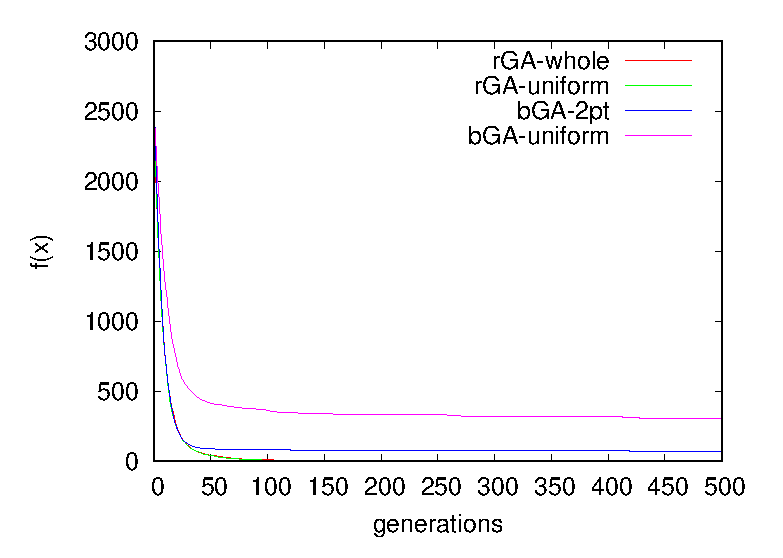
\includegraphics[width=\linewidth]{fig/cmp4GA/4GAs.eps}}
\centerline{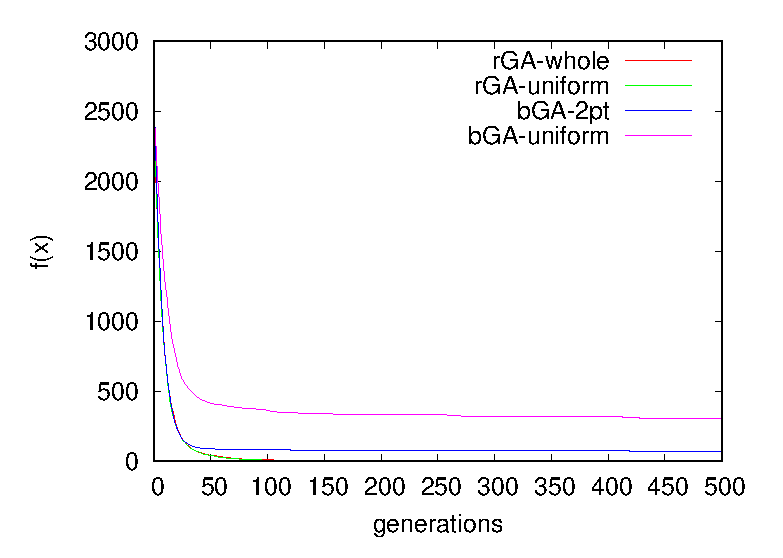
\includegraphics[width=7.5cm]{fig/cmp4GA/4GAs.eps}}
\caption{Anytime behavior (averaged over 30 trials) of the above GAs}
\label{fig}
\end{figure}

\section{Comparison}
Compare convergence speed and solution quality between different representations and operators; give reasons why some combination performs better (or worse).

\subsection{Convergence Speed}
Real-valued GAs and Binary GA with 2-point crossover have same speed at the begin, and Binary GA with 2-point crossover converge first, then the 2 Real-valued GAs converge, then the Binary GA with uniform crossover.

\subsection{Solution Quality}
Real-valued GAs have better performance over the 4 GAs, and they could reach the optimum f(x) value (0). However, Binary GAs can't reach the optimum f(x) value, and Binary GA has the worst performance

\subsection{Description}
The representation of the above GAs lead to these outcomes. For Binary GAs, changing of bits would have different degrees of influence due to it's location. Take 0000000000 as example, this gene has it's fitness -512, if the first bit changes to 1 (1000000000), then value would be 0, in the meanwhile, the change of last (0000000001) bit would only lead to the change of 1. And for Real-valued GAs the method of crossover would lead the children be the mid-fitness of their parents, thus would tend to evolute into the mid-point of the search space, which is 0 the optimum point. Thus Real-valued GAs would have better convergence speed and solution quality in this problem.

\section{Other Setting}
In this section, I had tried different parameters setting for $p_{c}, p_{m}, n$, and different settings have different effect on diffent method: 

\subsection{Binary GA(Uniform Crossover)}
\begin{description}
\item [$p_{c}$] Owing to the symmetrical characteristics of the uniform crossover, the anytime behaviors are the alike with $p_c$ and $(1-p_c)$, and $p_c=0.5$ converged faster and performed better than others.
\item [$p_{m}$] Mutation rate would take effect on both convergence speed and solution quality. In the experiment, $p_m=0.05$ is the best parameter setting for the uniform crossover binary GA.
\item [$n$] In this experiment $n=1$(ramdon selection) converge slower but have better solution quality.
\end{description}

\begin{figure}[htbp]
\centerline{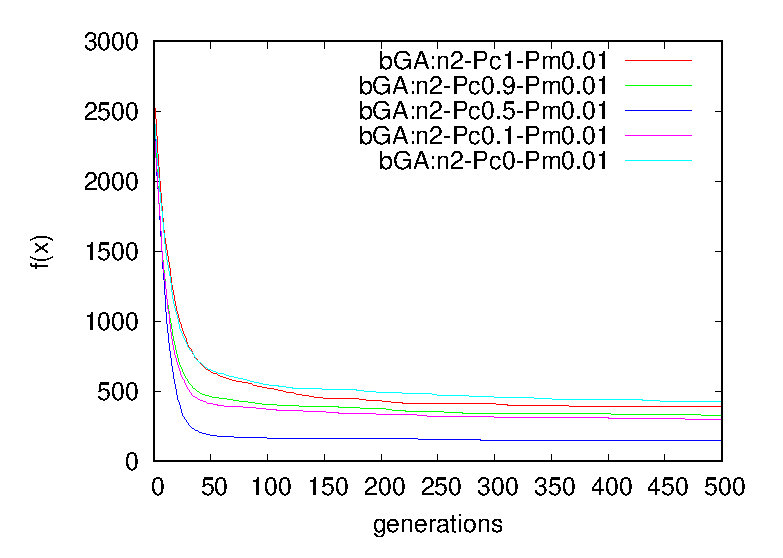
\includegraphics[width=7.5cm]{fig/bGA/change_pc_uni.eps}}
\caption{Binary GA(Uniform Crossover) with different $p_{c}$.}
\label{fig}
\end{figure}

\begin{figure}[htbp]
\centerline{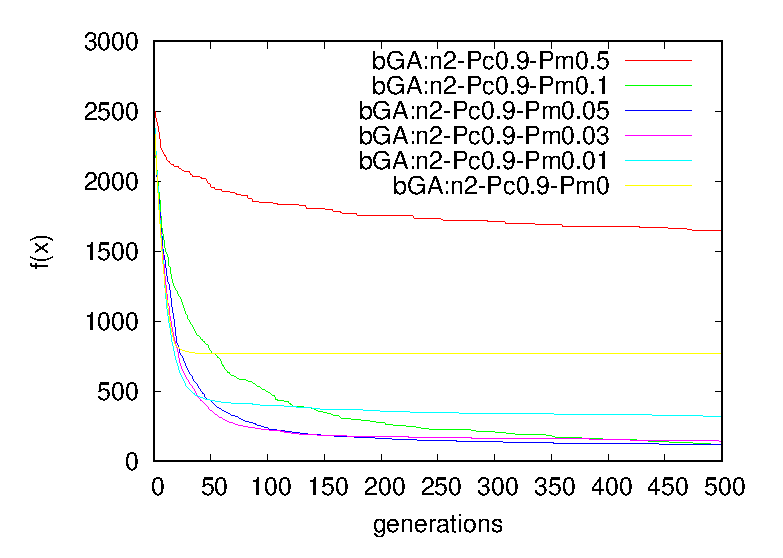
\includegraphics[width=7.5cm]{fig/bGA/change_pm_uni.eps}}
\caption{Binary GA(Uniform Crossover) with different $p_{m}$.}
\label{fig}
\end{figure}

\begin{figure}[htbp]
\centerline{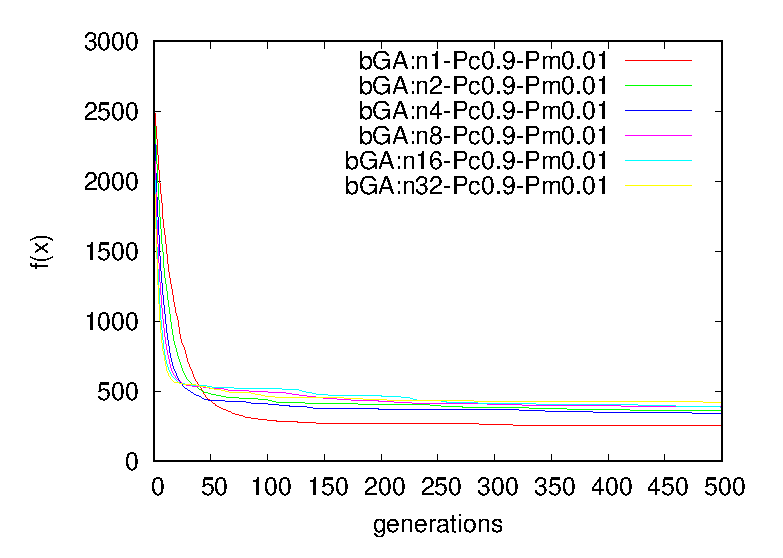
\includegraphics[width=7.5cm]{fig/bGA/change_n_uni.eps}}
\caption{Binary GA(Uniform Crossover) with different $n$-Tournament size.}
\label{fig}
\end{figure}

\subsection{Binary GA(2-point Crossover)}
\begin{description}
\item [$p_{c}$] Convergence speed are same, and the higher the crossover rate the better solution quality.
\item [$p_{m}$] Higher or zero mutation rate would lead to slowlier convergence speed.
\item [$n$] In this experiment $n=1$(ramdon selection) converge slower but have better solution quality.
\end{description}

\begin{figure}[htbp]
\centerline{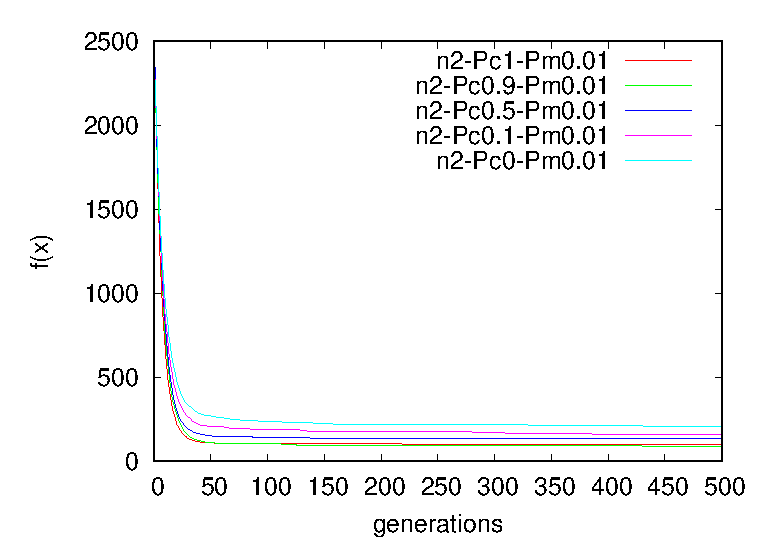
\includegraphics[width=7.5cm]{fig/bGA/change_pc_2pt.eps}}
\caption{Binary GA(2-point Crossover) with different $p_{c}$.}
\label{fig}
\end{figure}

\begin{figure}[htbp]
\centerline{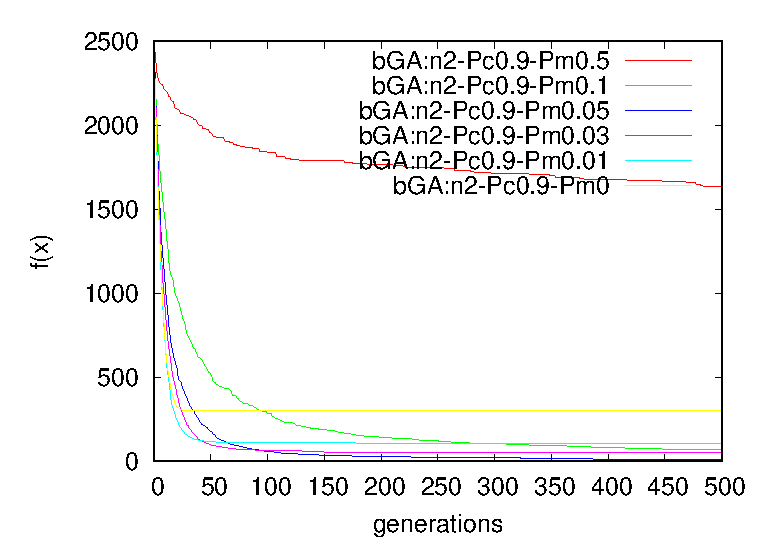
\includegraphics[width=7.5cm]{fig/bGA/change_pm_2pt.eps}}
\caption{Binary GA(2-point Crossover) with different $p_{m}$.}
\label{fig}
\end{figure}

\begin{figure}[htbp]
\centerline{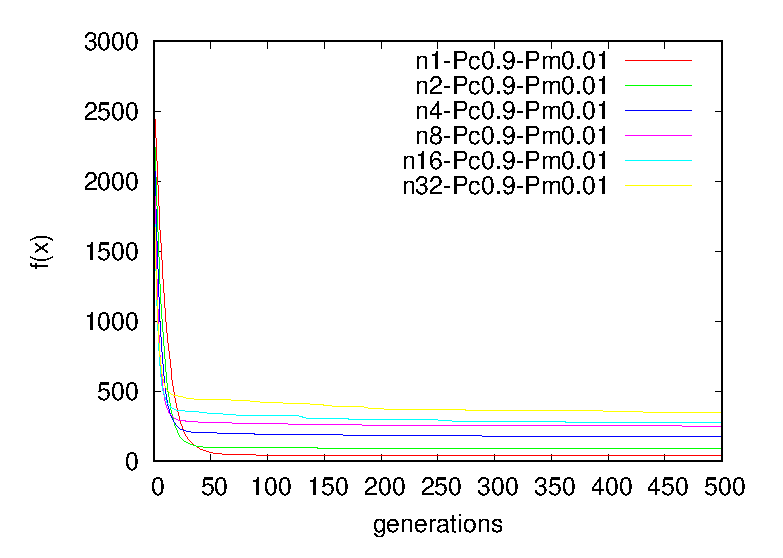
\includegraphics[width=7.5cm]{fig/bGA/change_n_2pt.eps}}
\caption{Binary GA(2-point Crossover) with different $n$-Tournament size.}
\label{fig}
\end{figure}

\subsection{Real-valued GA(Uniform Crossover)}
\begin{description}
\item [$p_{c}$] Both settings could get the optimum solution, and the higher crossover rate the faster convergence speed.
\item [$p_{m}$] Zero mutation rate would converge too fast thus had poor solution quality.
\item [$n$] Both settings could get the optimum solution, and the higher $n$-Tournament selection the faster convergence speed.
\end{description}

\begin{figure}[htbp]
\centerline{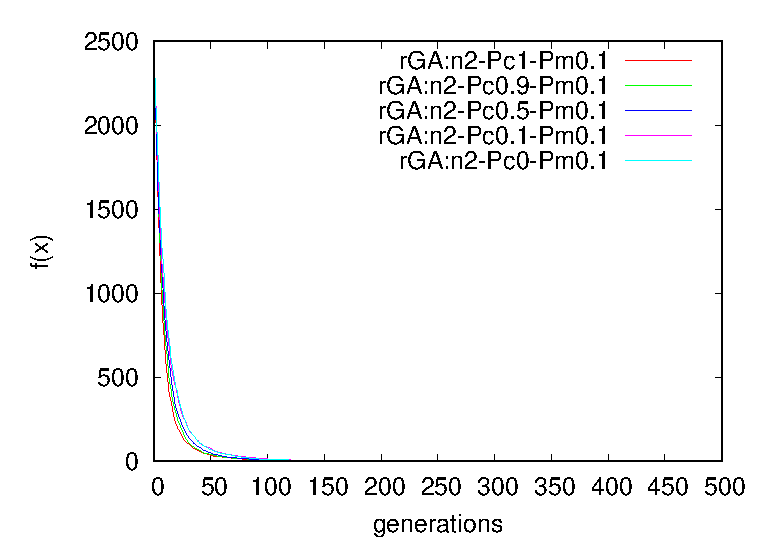
\includegraphics[width=7.5cm]{fig/rGA/change_pc_uni.eps}}
\caption{Real-valued GA(Uniform Crossover) with different $p_{c}$.}
\label{fig}
\end{figure}

\begin{figure}[htbp]
\centerline{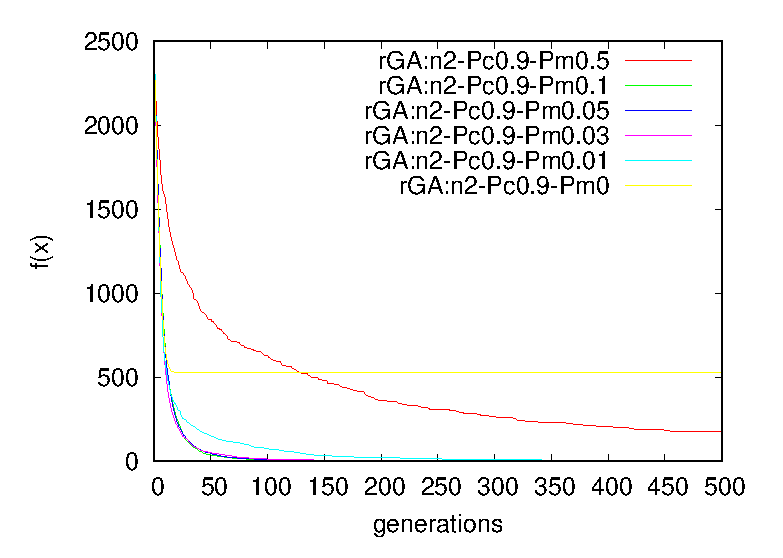
\includegraphics[width=7.5cm]{fig/rGA/change_pm_uni.eps}}
\caption{Real-valued GA(Uniform Crossover) with different $p_{m}$.}
\label{fig}
\end{figure}

\begin{figure}[htbp]
\centerline{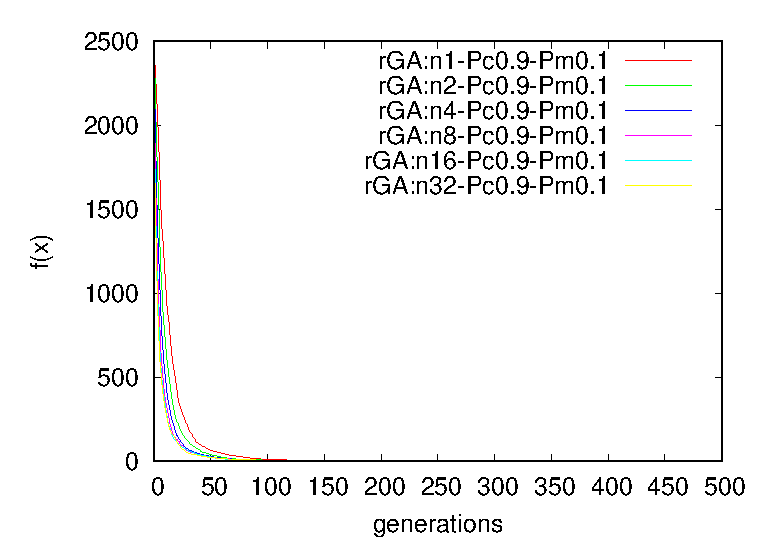
\includegraphics[width=7.5cm]{fig/rGA/change_n_uni.eps}}
\caption{Real-valued GA(Uniform Crossover) with different $n$-Tournament size.}
\label{fig}
\end{figure}

\subsection{Real-valued GA(Whole Arithmetic Crossover)}
\begin{description}
\item [$p_{c}$] Both settings could get the optimum solution, and the higher crossover rate the faster convergence speed.
\item [$p_{m}$] Zero mutation rate would converge too fast, thus had poor solution quality. The higher mutation rate would cause it converge slowlier.
\item [$n$] Both settings could get the optimum solution, and the higher $n$-Tournament selection the faster convergence speed.
\item [$\alpha$] Different $\alpha$ settings for whole Arithmetic Crossover seems to heve no effect on the result. 
\end{description}

\begin{figure}[htbp]
\centerline{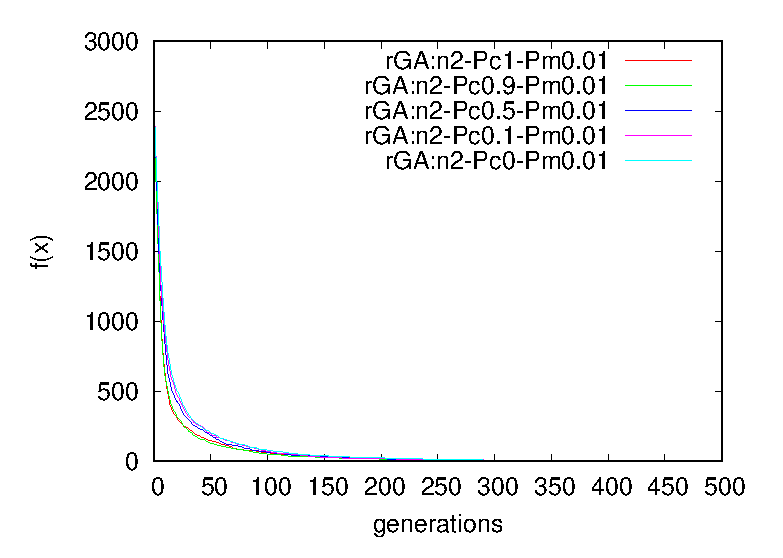
\includegraphics[width=7.5cm]{fig/rGA/change_pc_whole.eps}}
\caption{Real-valued GA(Whole Arithmetic Crossover) with different $p_{c}$.}
\label{fig}
\end{figure}

\begin{figure}[htbp]
\centerline{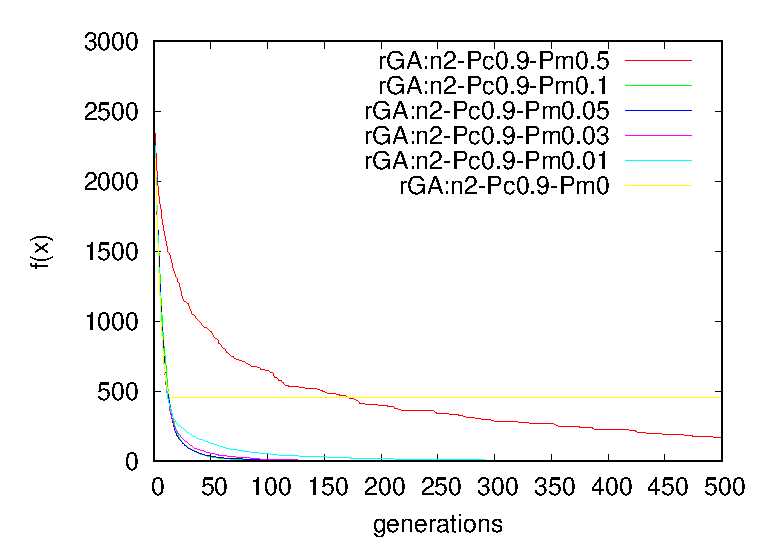
\includegraphics[width=7.5cm]{fig/rGA/change_pm_whole.eps}}
\caption{Real-valued GA(Whole Arithmetic Crossover) with different $p_{m}$.}
\label{fig}
\end{figure}

\begin{figure}[htbp]
\centerline{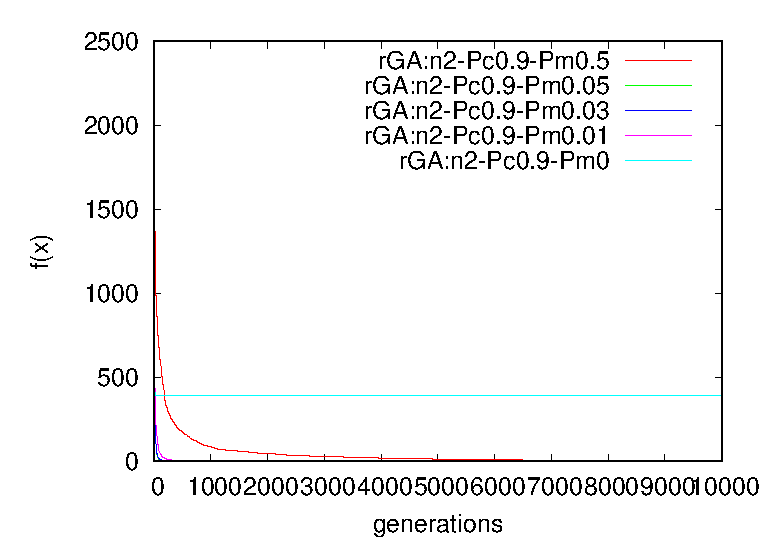
\includegraphics[width=7.5cm]{fig/rGA/change_pm_whole10000.eps}}
\caption{Real-valued GA(Whole Arithmetic Crossover) with different $p_{m}$ (10000 generations).}
\label{fig}
\end{figure}

\begin{figure}[htbp]
\centerline{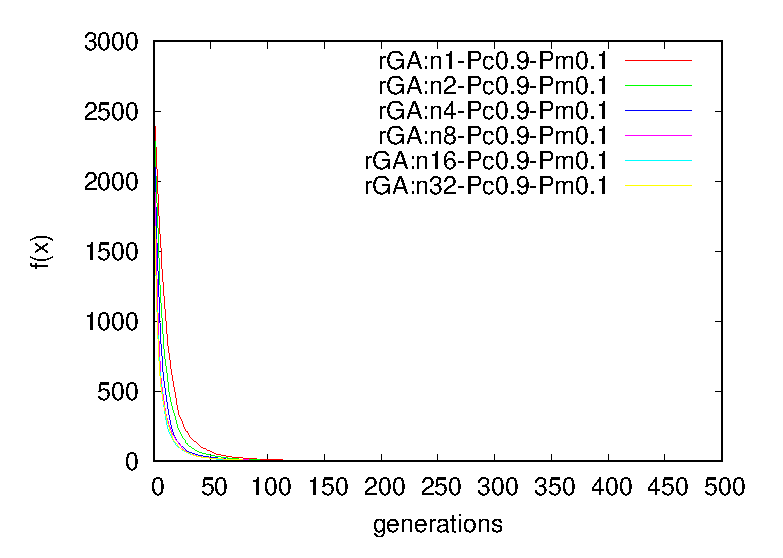
\includegraphics[width=7.5cm]{fig/rGA/change_n_whold.eps}}
\caption{Real-valued GA(Whole Arithmetic Crossover) with different $n$-Tournament size.}
\label{fig}
\end{figure}

\begin{figure}[htbp]
\centerline{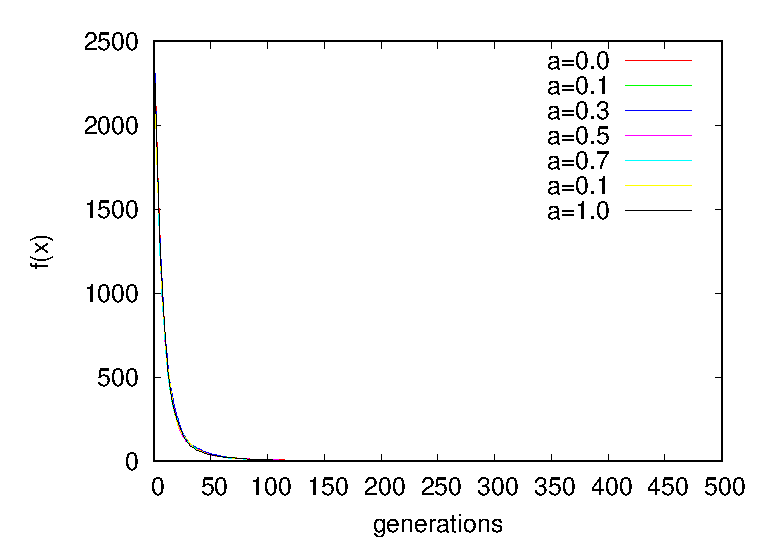
\includegraphics[width=7.5cm]{fig/rGA/change_a_whole.eps}}
\caption{Real-valued GA(Whole Arithmetic Crossover) with different $\alpha$ settings.}
\label{fig}
\end{figure}


\section{Large-scale Problem}
\begin{figure}[htbp]
\centerline{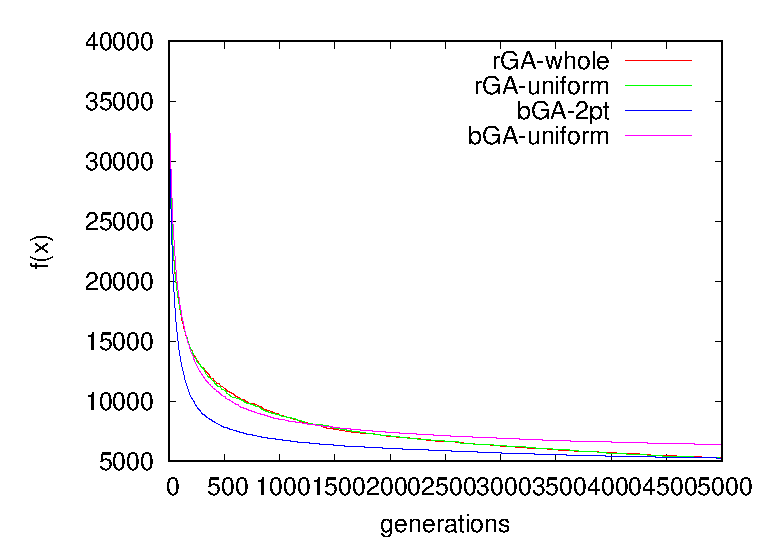
\includegraphics[width=7.5cm]{fig/cmp4GA/4GAs-N100.eps}}
\caption{Anytime behavior (averaged over 30 trials) of the above GAs for $N=100$.}
\label{fig}
\end{figure}


\vspace{12pt}
\end{CJK}
\end{document}
